\documentclass{article}
\usepackage{graphicx}
\usepackage{epsfig,epstopdf}
\usepackage{amssymb,amsmath,bm}
\usepackage{textcomp}
\usepackage{caption}
\usepackage{multirow}
\usepackage{nonfloat}
\usepackage{flushend}
%\usepackage{subfigure}
\usepackage{algorithm}
\usepackage{subcaption}
\usepackage{algorithmic}
\usepackage{url}
\usepackage{hyperref}
\usepackage{lipsum}

\DeclareMathSizes{10}{10}{10}{10}




\title{NLP Project Proposal}

\author{ {\bf Group 13} \\ Saranya .M .S (CS15D006), Sridharan Sankaran (CS14S024)}

\begin{document}
\maketitle

\section*{Project title}
{ \textit {Generating and reading the weather report from satellite images using image processing, data mining and Natural Language Generation techniques }}

\section*{Problem Definition}

In this project work a weather report is generated using image processing and data mining techniques 
and a text-to-speech synthesis system is used to read the report using synthesized 
voice. The navigation direction of cyclones and typhoons are predicted after processing
the satellite images. A look-up table with  list of near-by cities is generated with
their latitude and longitudinal values. A weather report is made with the calculated direction and speed of the cyclones along with the nearby cities. Text to speech
synthesis system is implemented using HMM based speech synthesis system to read this
text report for the blind people. 

\section{Proposed Approach}

\subsection{Introduction}
\label{sec:intro}
Weather forecasting become an essential thing in our daily life to know the upcoming 
natural calamities. With the advancement in the meteorology and communication 
technology, images obtained by the satellites stationed above are used in weather
forecasting. But the forecasting requires intense training and advanced education to 
interpret the information form the satellite pictures. Meteorological department has already
automated the gathering of satellite images in the database. Further advancement can be
brought by automating the weather forecasting. Although the automated forecast may not
be as accurate as the experts interpretation \cite{weatherReport}, Forecast Production Assistant (FPA) was 
developed to automate the routine aspects for public health and safety in hazardous
 weather \cite{fpa}. 

\subsection{Image database}
\label{sec:db}
The satellite images are gathered from Hong kong Observatory website located at http://www.hko.gov.hk/wxinfo/intersat/satellite/sate.htm. Here we consider deep convection weather images of Asia taken from satellites at intervals of about once every half-hour. Deep convection clouds are very dense with water content and  are seen as red patches in the images. Since the above mentioned website retains only the images of recent 3 days , we have a crone job that runs every hour and downloads these images to build a time series database of images. 

\subsection{Image processing}
\label{sec:imgProcessing}
These downloaded images are processed to track the movement of cyclones due to convection clouds. The various steps involved in tracking these cyclones are as below:

\subsubsection{Algorithm}
\label{ssec:algo_image}

\begin{algorithm}[!th]
\caption{Cyclone tracking algorithm}
\label{algo:img}
\begin{algorithmic}[1]

\STATE  \textbf{Input:} Images from HK observatory at 30 minutes interval\\
\textbf{Output:} Weather report as English language text 
\STATE Process input image to retain only those pixels corresponding the convection cloud movement
\STATE Find all the pixel values of resulting image
\STATE Retain only the red pixels corresponding to the convection clouds
\STATE Use DBSCAN algorithm to identify only those clusters (cyclones) that are big enough to be reported
\STATE Use k-means to find the centroids of these clusters (cyclones)
\STATE Track the movement of these centroids from one image to another as a time series data
\STATE Create weather report that locates the movement of the cyclone along with its speed using nearby city database lookup table
\end{algorithmic}
\end{algorithm}

\subsection{Look-up table}
\label{sec:lookupTable}

Generally weather prediction is globally classified into different sectors like East 
pacific, West pacific, Indian basin, Atlantic basin etc. Each sector will be monitored 
by a set of geo-stationary or mobile satellites. So each satellite may cover only 
limited area. The major cities falling under those sectors can be easily enlisted based 
on their latitude and longitude values. 

Since our database is around Hong Kong , the major 
cities and places in and around are identified and tabulated offline. This table acts a 
look-up table to include the city names and warn the people of those locality. The 
near-by victim of a hazardous climate can be calculated using the {\textit{Euclidean 
distance}} between the latitude and longitude of the cyclone and that of the cities 
listed in the look-up table.

\subsection{Text-based weather report}
\label{sec:textReport}

The navigation of cyclone determined by the movement of "eye-of-the-cyclone" and decoded 
in terms of eight directions (North, South, East, West, North-East, North-West, South-
East and South-West). The speed of the cyclone is calculated as the distance travelled by the eye over the time period. The latitude and longitude of the cyclone is also
obtained from the satellite image along with the direction as explained in Section \ref{sec:imgProcessing} and the cities in the path of cyclone are identified from the look-up table as detailed in Section \ref{sec:lookupTable}. These informations are appended in a text file immediately after analysing the satellite images. 
The text report will of this following sample format.

{\textbf{Example:} \textit{Cyclone-1 moves towards North-west direction with a speed of 120 kmph towards the city of Milinani}}

\subsection{Text-to-speech synthesis}
\label{sec:tts}
The process of generating text report from the image sequence itself in a NLG process. 
The text report is then read aloud using Text-to-speech (TTS) module, which is another 
NLG process in order to help the visually impaired people. Given a text in one language, 
a Text-to-Speech (TTS) system is expected to produce high quality speech signal
(corresponding to the text provided) which is intelligible to a human listener. TTS
is a well developed area which can be achieved in more than one way. Numerous research 
work had been carried out in the past to build a high quality speech synthesizer 
for one language. Speech synthesis is the process of introducing engineering approaches 
for "talking" machines that uses a sequence of sub-word units. The use of such elements
provide flexibility for vocabularies as required for applications like text to speech. This speech synthesis can be carried out in two different ways namely, (1) Unit Selection based speech Synthesis (USS) \cite{uss} and (2) Statistical parametric speech synthesis technique \cite{zenStatistical}.

Text-to-speech processing involves three phases as mentioned below
\begin{itemize}
\item {\bf Text preprocessing:} This step translates the text string of characters into
a new string with resolved ambiguities.
\item {\bf Text to phonetic translation:} The processed text is parsed to determine
phonetic structure. A sequence of modifications to canonical pronunciations is typically
encoded in a series of rewrite rules.
\item {\bf Speech synthesis:} Given the sequence of quantities like pitch, duration, amplitude along with unit label, the signal processing component generates speech.
\end{itemize}

\begin{figure}[h]
\centering
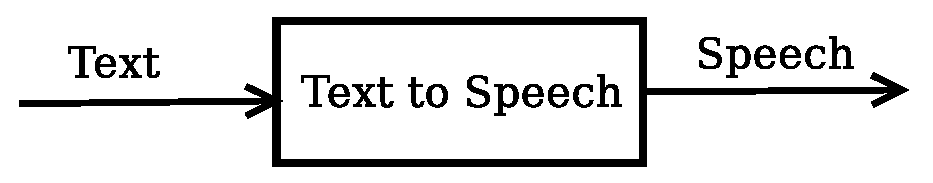
\includegraphics[scale=0.35]{figures/tts.eps}
\caption{Text to speech synthesis process}
\label{fig:ttsBlock}
\end{figure}

\subsubsection{HMM-based speech synthesis}
\label{ssec:hmm}
Hidden Markov Models (HMMs) can be used to model any time series. HMM tool kit (HTK) developed by Microsoft and Cambridge University is used to build HMMs. Initially HTK was
designed for building HMM-based speech processing tools, in particular recognizers. As 
shown in the picture above, there are two major processing stages involved. Firstly, the HTK training tools are used to estimate the parameters of a set of HMMs using training
utterances and their associated transcriptions. Secondly, unknown utterances are
transcribed using the HTK recognition tools.

\begin{figure}[h]
\centering
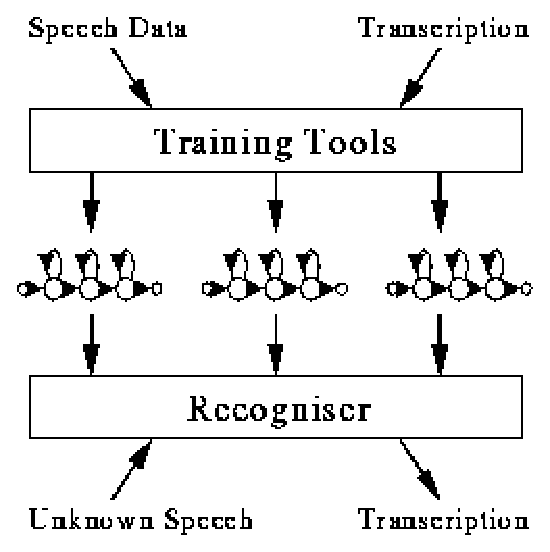
\includegraphics[scale=0.45]{figures/htk_overview.eps}
\caption{Overview of HTK}
\label{fig:htkOverview}
\end{figure}

\subsection{Speech Corpus}
For developing a TTS system, we need the recorded speech content, generally called
as speech corpus which serves as a database. The text-to-Speech synthesis process needs
two types of data namely, 1) Text data and 2) Speech data. The former one is the text
form of the content which is to be recorded to get the later form of data. Here for the 
purpose of developing a phoneme-based speech synthesis model of English language, one
hour of CMU-artic corpus is used. The speech utterances in this database is recorded in 
studio environment with the sampling rate of 16KHz and 16 bit quantization.

The complete process of HMM-based speech synthesis system, shortly called as HTS 
(H-Triple-S) for a phoneme-level system is explained in Section \ref{ssec:tts_algo}.

\subsubsection{Algorithm}
\label{ssec:tts_algo}

\begin{algorithm}[!th]
\caption{Steps for text-to-speech using HTS }
\label{algo:hts}
\begin{algorithmic}[1]

\STATE  \textbf{Input:} Sentence(s) as text \\
\textbf{Output:} Synthesised speech
\STATE Prepare the speech corpus.
\STATE Pre-process the text data.
\STATE Segmentation and labelling of audio segments in corpus.
\STATE Manual correction of segmentation.
\STATE Preprocessing to get the phoneme labels.
\STATE Model training in HMM Training phase.
\STATE Verification of trained models.
\STATE HMM synthesis phase.
\end{algorithmic}
\end{algorithm}

\section{Evaluation Measures}
\label{sec:evalMeasures}
The first process of this project are image processing which analysis the image sequence
of climatic conditions and creates a weather report as text document with the location, direction, and speed of the cyclones. The accuracy of 
\begin{itemize}
\item the cyclone location with latitude and longitude
\item the direction of the cyclone movement
\item the speed of the cyclone movement
\item identifying the near-by or next hit areas in terms of city names
\end{itemize} are to be evaluated. This can be done by comparing the manually prepared report and the report generated by the automated process for the validation image set.

The second part of the project is to generate the synthesised voice from the text report. The synthesised voice has to be evaluated for 
\begin{itemize} 
\item intelligibility and 
\item naturalness.
\end{itemize} 
This can be evaluated by a measure called "Mean Opinion Score" (MOS) \cite{mos}.
This score is calculated by playing the natural human speech and the synthesised speech alternatively to a set of naive speakers and asking them to give scores in the scale of 1 to 5 to measure the intelligibility and naturalness of the synthesised speech. The scale of 1 to 5 has the standard meaning as given below.
\begin{table}[h]
\centering
\begin{tabular}{|c|l|l|}
\hline 
{\bf MOS	} & {\bf Quality } & {\bf Impairment} \\
\hline
5 & Excellent	& Imperceptible \\
4	& Good	& Perceptible but not annoying \\
3	& Fair	& Slightly annoying \\
2	& Poor	& Annoying \\
1	& Bad	& Very annoying \\ 
\hline 
\end{tabular}
\vspace{2mm}
\caption{Mean opinion score (MOS)}
\label{tab:mosDefn}
\end{table}



\clearpage 

\bibliographystyle{IEEEtranS}
\bibliography{refs}


\end{document}
